\chapter{Additional notes to CT-like Controllers}

This chapter will provide some additional remarks to the computed torque like controllers with gravity compensation, which can be seen in figure \ref{fig:ctLike_overview}. This controller has, compared to the computed torque controller in figure \ref{fig:ct_overview}, only the gravitational term in the linearizing component.


\begin{figure}[H]
	\centering
	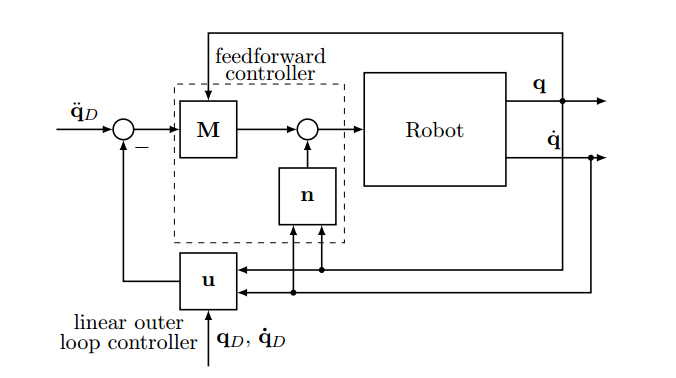
\includegraphics[width=0.85\textwidth]{pics/ct_controller.png}\\
	\caption{Controller overview of Computed Torque controller}
	\label{fig:ct_overview}
\end{figure}


\begin{figure}[H]
	\centering
	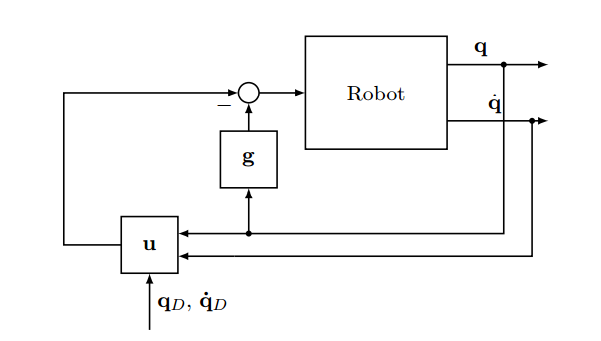
\includegraphics[width=0.65\textwidth]{pics/gravityController.png}\\
	\caption{Controller overview of Computed Torque like controller with gravity compensation}
	\label{fig:ctLike_overview}
\end{figure}

This type of controller has shown good behavior, even though there have been a lot of simplifications within th design process. The terms which have been excluded are the inertia term and the centrifugal/coriolis part. If the application or the architecture of the robot is chosen, so that the excluded terms have almost no influence of the final dynamics, this approach become even more suitable. An example for such a layout/application is a robot arm which is not moving a lot, and is controlling for a steady state position most of the time. In this case the centrifugal term becomes irrelevant and since the robot does not see a lot of acceleration the inertia term can also be ignored.\\[1cm]

Comment to the PD Control within figure 3.6 (p.17):
The proper tracking of the reference with the aggressive parameter set is bought with unrealistic high torque vales. The peak for the first joint is around 250Nm. Values in this range does require huge motors and might even be higher then the mechanical stability of the robot arm, which is by given as a lightweight one.

